\documentclass[aspectratio=169, 12pt]{beamer}    %set the aspect ratio to 16:9
%\documentclass[]{beamer}  %set the aspect ratio to 4:3

\usepackage[dct]{AUTtheme}     % AUT theme                                  
                                 
% title page content
\title[Beamer title]
{Creating Slides Using Beamer \\ and the AUTtheme
}
\subtitle{A user guide}
\author[Sarah, Wenqiang]{Sarah Marshall\inst{1}, Wenqiang Liu\inst{2}}
\institute
{\inst{1}  Engineering, Computer Mathematical Sciences (ECMS) \\
\inst{2}  Engineering, Computer Mathematical Sciences (ECMS) 
%\inst{3}  Engineering, Computer Mathematical Sciences (ECMS) 
}
\date{
%The Name of the Conference \\ The Name of the Venue \\
17 April 2023
}
 
\bibliographystyle{plain}

\begin{document}

\begin{frame}
    \maketitle
\end{frame}


\begin{sectionframe}
\frametitle{Table of Contents}
\tableofcontents[hideallsubsections]
\end{sectionframe}



\section{Frames}


\subsection{Frame Sizes}
\begin{frame}[fragile = singleslide]{Frame Sizes}

The template can be used to create $16\times9$ or $4 \times 3$ slides.
The resolution of the background images get updated automatically.

\begin{itemize}
\item To create $16 \times 9$ slides
\begin{verbatim}
\documentclass[aspectratio=169]{beamer} 
\end{verbatim}

\item To create $4 \times 3$ slides
\begin{verbatim}
\documentclass[]{beamer}  
\end{verbatim}

\end{itemize} 


\end{frame}

\subsection{Loading the AUTTheme}
\begin{frame}[fragile = singleslide]{Loading the AUTTheme}
 
\begin{verbatim}
\usepackage{AUTtheme}  
\end{verbatim}

The DCT colour theme is the default, however it can be forced as follows:
\begin{verbatim}
\usepackage[dct]{AUTtheme}  
\end{verbatim}


\end{frame}

\subsection{Compiling with AUTTheme}
\begin{frame}[fragile = singleslide]{Compiling with AUTTheme}
 
\verb|lualatex| is recommended.

\end{frame}



\subsection{Frame Types}
\begin{frame}[fragile = singleslide]{Frame Types}

This template uses three types of frames
\begin{itemize}
 \item \alert{Title page:}
 \begin{verbatim}
\begin{frame}
  \maketitle 
\end{frame}
\end{verbatim}
 
 \item \alert{Section frame:}
 \begin{verbatim}
\begin{sectionframe}\frametitle{Frame Title}
 Content for right hand side of slide
\end{sectionframe}
\end{verbatim}

\item \alert{Default frame:}
\begin{verbatim}
\begin{frame}{Frame Title}
Frame content
\end{frame}
\end{verbatim}

\end{itemize}
\end{frame}


% \begin{frame}[fragile]{How to create title page}
%   A title page can be created the traditional way, using the "maketitle" or "titlepage" commands in a frame environment.

% \begin{columns}
%     \column{0.6\textwidth}
%     \begin{alertblock}{Method two}
%     \begin{verbatim}
%     \begin{titleframe}
%         \maketitle
%     \end{titleframe}
%     \end{verbatim}
%     \end{alertblock}
%     \column{0.4\textwidth}
%         You can build a title page based on this code in the box on the left side.
% \end{columns}
% \end{frame}

\subsection{New sectionframe environment}
\begin{frame}[fragile]{Create contents page using sectionframe environment}
\begin{columns}
\column{0.6\textwidth}
\begin{alertblock}{Example Code}

\begin{verbatim}
\begin{sectionframe}
\frametitle{Table of Contents}
\tableofcontents[
     hideallsubsections]
\end{sectionframe}
\end{verbatim}

\end{alertblock}

\column{0.4\textwidth}
 You can use \verb|\tableofcontents| or build your own table of contents page.
\end{columns}
\end{frame}


\begin{frame}[fragile]{Slides at beginning of section}

By default two \verb|sectionpage| is displayed at the start of each section.
The first contains the section name and the second contains 
 a table of contents.

Both can be edited within the \verb|.tex| file.

e.g. To switch off use within the \verb|.tex| file.
\begin{verbatim}
\AtBeginSection{}
\end{verbatim}



\end{frame}

\section{Slide Content}



\subsection{Bulleted lists}
\begin{frame}[fragile]{List}
    \begin{itemize}
        \item Item 1
        \begin{itemize}
            \item Subitem 1.1
            \begin{itemize}
                \item Subsubitem  1.1.1
                \item Subsubitem 1.1.2
            \end{itemize}
%            \item Text visible on slide 1.2
%            \begin{itemize}
%                \item Text visible on slide 1.2.1
%                \item Text visible on slide 1.2.2
%            \end{itemize}
        \end{itemize}
        \item<2-> Item 2 -- This item appears second due to \verb|<2->|
        \item Item 3
        % \item Text visible on slide 4
        % \item Text visible on slide 5
    \end{itemize}
\end{frame}



\begin{sectionframe}
    \frametitle{Example: create a one-off table of contents}
    \setlength{\parskip}{0ex}
\tableofcontents[ 
    	currentsubsection, 
        sectionstyle=show/shaded, 
        subsectionstyle=show/show/hide,
    ] 
    

 
\end{sectionframe}

\subsection{Ordered Lists}
\begin{frame}[fragile]{Ordered Lists}
    \begin{enumerate}%[default]
    \item Point 1 
    \item Point 2 
    \begin{enumerate}[a.]
        \item part a 
            \begin{enumerate}[i.]
                \item another point
                \item another point
            \end{enumerate} \pause
        \item The \verb|\pause| command can be used to delay appearance of content 
            \begin{itemize}%[i]
                \item another point
                \item another point
            \end{itemize}
    \end{enumerate}
    \item Point 3 
    \item Point 4 
    \end{enumerate}
\end{frame}



\subsection{Highlights and Colours}
\begin{frame}[fragile]{Highlights and Colours}

\begin{itemize}
\item 
    \colorbox{orange}{highlighted}  \verb|\colorbox{orange}{text}|
\item     
     \alert{AUT-themed orange text}  \verb|\alert{text}| or \verb|\textcolor{deeporangeAUT}{text}|.    
\item  \textbf{bold} \verb|\textbf{text}|
\item  \alert{alert} \verb|\alert{text}|
\item  \textcolor{blue}{coloured} \verb|\textcolor{blue}{text}|
  

\end{itemize}
    
    
\end{frame}

\subsection{Blocks}
\begin{frame}{Blocks}
        %  alert block
    \begin{alertblock}{Alert block}
        This is an alert block, customised to match the AUT colour scheme.
        
    \end{alertblock}
    
    \begin{block}{Block}
        This is a standard block.
    \end{block}  

    \begin{exampleblock}{Example block}
        This is an example block.
    \end{exampleblock}  

\end{frame}


\subsection{Columns}
\begin{frame}{Columns}
     % Get the performance of column
    \begin{columns}
    \column{0.5\textwidth}
    This is a text in the first column.
    $$E = mc^2 $$
    \begin{itemize}
        \item The first term
        \item The second term
    \end{itemize}
    
    \column{0.5\textwidth}
    This is a text in the second column.
    \end{columns}
\end{frame}

% in three columns
\begin{frame}{Three columns}
    \begin{columns}
        \column{0.3\textwidth}
        This is the first column content.
        \column{0.3\textwidth}
        This is the second column content.
        \column{0.3\textwidth}
        This is the third column content.
    \end{columns}
\end{frame}


\subsection{Citations and Footnotes}
\begin{frame}{Citations and Footnotes}
You can cite a paper like this \cite{teichmann2019machine, buehler2019deep}. 

Footnotes can be inserted like this
\footnote[frame]{
Lam, Yeh. The Geometric Process and Its Applications. World Scientific, Hackensack,
NJ, 2007.
}.
\end{frame}

\section{Maths and Floats}
\subsection{Mathematical formula}
\begin{frame}{Using math formula}
In this slide, we insert an equation(\ref{E1}), which is the definition of $y$.
\begin{equation}
    \label{E1}
    y = 
    \begin{cases}
    \frac{1}{f(x)},\ f(x) \neq 0 \\
    f(x), \ f(x) = 0
    \end{cases}
\end{equation}
\end{frame}


\subsection{Tables}
\begin{frame}
\frametitle{Insert a table}
This results are shown in Table \ref{T1}
\begin{table}[ht]   
    \caption{A sample table}
    \label{T1}
    \centering
    \begin{tabular}{p{1.5cm}|p{1.5cm}|p{1.5cm}}
    \hline
    Metrics     &   M1      &   M2      \\
    \hline
    Accuracy    &   84\%    &   88\%     \\
    Precision   &   91\%    &   90\%     \\
    Recall      &   75\%    &   77\%     \\
    \hline
    \end{tabular}
\end{table}
\end{frame}

\subsection{Figures}
\begin{frame}{Insert a sample figure}
The data-set information is shown in Figure \ref{fig:dataset}.
\begin{figure}
    \centering
    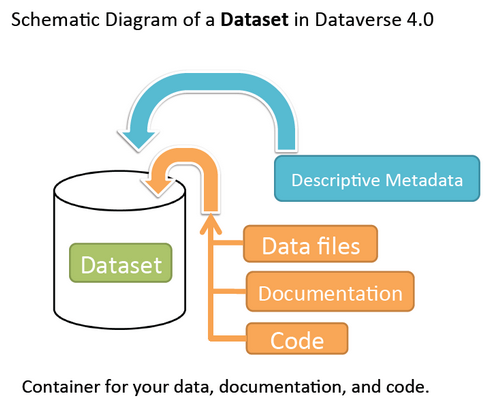
\includegraphics[width=6cm,height=4.5cm]{figs/dataset.png}
    \caption{A sample picture}
    \label{fig:dataset}
\end{figure}
\end{frame}

\section*{References}

\begin{frame}{References}
% Show the references
\bibliography{bib}
\end{frame}

\begin{sectionframe}

\begin{center}
{\Huge
\alert{
Thank you very much for your attention!
}
}
\end{center}
\end{sectionframe}


\begin{titleframe}
\begin{center}
{
\huge

\vspace{1cm}

\textcolor{white}{
The end
}
\vspace{1cm}

}
\end{center}
\end{titleframe}

\begin{titleframe}
\end{titleframe}


\end{document}

